
\documentclass{beamer}

\mode<presentation> 
  {
  \usetheme{Madrid}
  }

%%%%%%%%%%%%%%%%%%%%%%%%%%%%%%%%%%%%% PAQUETES %%%%%%%%%%%%%%%%%%%%%%%%%%%%%%%%%%%%%%%%%%

\usepackage[utf8]{inputenc}
\usepackage[spanish]{babel}
\usepackage[T1]{fontenc}
\usepackage{graphicx}
\usepackage{dsfont} % inclusion de R^n
\usepackage{animate} % para crear el gif de kmeans
\decimalpoint % cambia la coma por el punto como separador de decimales en math mode
\usepackage{listings} % para el codigo fuente
\lstset
  {
  basicstyle=\footnotesize,
  commentstyle=\color{green}, % Estilo de los comentarios
  }
\usepackage{hyperref} % para las referencias cruzadas
\hypersetup
{
    pdfstartview={Fit},      % fits the width of the page to the window
    pdftitle={Estudio comparativo de Algoritmos de machine learning e implementación en Hadoop},    % title
    pdfauthor={David Retana Ribeiro},     % author
    pdfsubject={Big data y machine learning},   % subject of the document
    pdfkeywords={computacion paralela, apache hadoop, apache spark, machine learning, big data, python, k means, cluster},
    pdfnewwindow=true,      % links in new PDF window
    colorlinks=true,       % false: boxed links; true: colored links
    urlcolor=cyan           % color of external links
}

%%%%%%%%%%%%%%%%%%%%%%%%%%%%%%%%%%%%%% TITULO %%%%%%%%%%%%%%%%%%%%%%%%%%%%%%%%%%%%%%%%%%%

\title[Machine Learning y Big Data]
      {Estudio comparativo de algoritmos paralelos de machine learning e implementación en Hadoop}
\author{David Retana Ribeiro}
\institute[UCM]{Universidad Complutense de Madrid \\ \medskip \texttt{davidret@ucm.es}}
\date{4 de Octubre de 2017}

%%%%%%%%%%%%%%%%%%%%%%%%%%%%%%%%%%%%%%%%%%%%%%%%%%%%%%%%%%%%%%%%%%%%%%%%%%%%%%%%%%%%%%%%%

\begin{document}

%%%%%%%%%%%%%%%%%%%%%%%%%%%%%%%%%%%%%%%%%%%%%%%%%%%%%%%%%%%%%%%%%%%%%%%%%%%%%%%%%%%%%%%%%

\begin{frame} % Portada
\titlepage
\end{frame}

%%%%%%%%%%%%%%%%%%%%%%%%%%%%%%%%%%%%%%%%%%%%%%%%%%%%%%%%%%%%%%%%%%%%%%%%%%%%%%%%%%%%%%%%%%

\begin{frame} % Indice de contenidos
\frametitle{Índice de contenidos}
\tableofcontents
\end{frame}

%%%%%%%%%%%%%%%%%%%%%%%%%%%%%%%%%%%%%%%%%%%%%%%%%%%%%%%%%%%%%%%%%%%%%%%%%%%%%%%%%%%%%%%%%%
%%%%%%%%%%%%%%%%%%%%%%%%%%%%%%%%%%%% INTRODUCCION %%%%%%%%%%%%%%%%%%%%%%%%%%%%%%%%%%%%%%%%
%%%%%%%%%%%%%%%%%%%%%%%%%%%%%%%%%%%%%%%%%%%%%%%%%%%%%%%%%%%%%%%%%%%%%%%%%%%%%%%%%%%%%%%%%%

\section{Introducción}

\begin{frame} % Introduccion a Big data y machine learning
  \frametitle{Introducción}
  \begin{block}{Big Data}
  \begin{itemize}
    \item Era de los datos.
    \item Conjunto masivo.
    \item Incapacidad de los sistemas tradicionales para manejar dichos datos.
  \end{itemize}
  \end{block}
  
  \begin{block}{Machine Learning}
  \begin{itemize}
    \item Rama de la inteligencia artificial.
    \item Sistemas que aprenden automáticamente sin ser programados específicamente para ello.
    \item El algoritmo o modelo aprende los patrones de los datos.
    \item Se apoya en las matemáticas para construir los modelos.
    \item Aprendizaje supervisado y aprendizaje no supervisado.
  \end{itemize}
  \end{block}
\end{frame}

%%%%%%%%%%%%%%%%%%%%%%%%%%%%%%%%%%%%%%%%%%%%%%%%%%%%%%%%%%%%%%%%%%%%%%%%%%%%%%%%%%%%%%%%%%

\begin{frame} % Como encajan Hadoop, mapreduce, spark y machine learning al big data
  \frametitle{Apache Hadoop y Apache Spark}
  \centering
  
\includegraphics[width=0.5\textwidth]{C:/Users/David/Desktop/TFG/TFGLatex/presentacion/recursos/mapreduce_logo.jpg}\\
  Actualmente, existen diversas herramientas que nos permiten trabajar con las grandes cantidades de datos
  manejadas en el \textit{Big Data}.
  
\includegraphics[width=0.5\textwidth]{C:/Users/David/Desktop/TFG/TFGLatex/presentacion/recursos/hadoop_logo.png}%
  
\includegraphics[width=0.5\textwidth]{C:/Users/David/Desktop/TFG/TFGLatex/presentacion/recursos/spark_logo.png}
\end{frame}

%%%%%%%%%%%%%%%%%%%%%%%%%%%%%%%%%%%%%%%%%%%%%%%%%%%%%%%%%%%%%%%%%%%%%%%%%%%%%%%%%%%%%%%%%%
%%%%%%%%%%%%%%%%%%%%%%%%%%%%%%%% DESPLIEGUE HADOOP %%%%%%%%%%%%%%%%%%%%%%%%%%%%%%%%%%%%%%%
%%%%%%%%%%%%%%%%%%%%%%%%%%%%%%%%%%%%%%%%%%%%%%%%%%%%%%%%%%%%%%%%%%%%%%%%%%%%%%%%%%%%%%%%%%

\section{Despliegue de un \textit{cluster Hadoop}}

\begin{frame} % imagen de topologia de un cluster Hadoop
\frametitle{Topología de un cluster Hadoop}
\begin{figure}
\centering
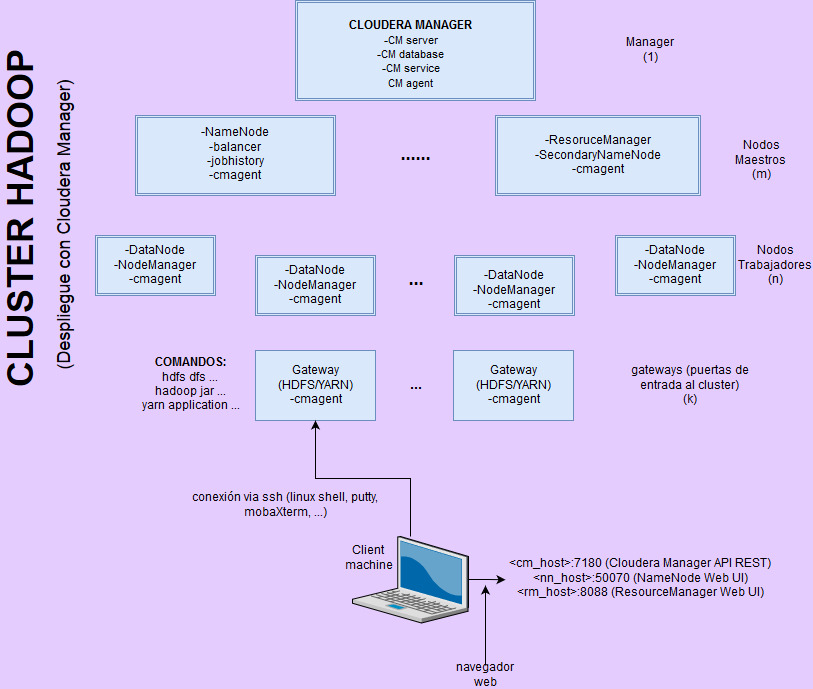
\includegraphics[scale=0.3]{C:/Users/David/Desktop/TFG/TFGLatex/imagenes/hadoop_topology.jpg}
\end{figure}
\end{frame}

%%%%%%%%%%%%%%%%%%%%%%%%%%%%%%%%%%%%%%%%%%%%%%%%%%%%%%%%%%%%%%%%%%%%%%%%%%%%%%%%%%%%%%%%%%

\subsection{\textit{HDFS} y \textit{YARN}}

\begin{frame}[fragile] % fragile permite añadir codigo con lstlisting
\frametitle{HDFS}
\begin{block}{Hadoop Distributed File System}
Ejemplos de comandos de HDFS:
\begin{lstlisting}[language=bash, numbers=none, frame=single]
$ # crea un directorio recursivamente
$ hdfs dfs -mkdir -R <direccion_a_crear>
$ # sube un archivo de local a HDFS
$ hdfs dfs -put <path_archivo_local> <path_hdfs> 
$ # Descarga un archivo de HDFS a local
$ hdfs dfs -get <path_hdfs> <path_local> 
\end{lstlisting}
\end{block}

En un navegador escribimos: \path{<ip_namenode>:50070}

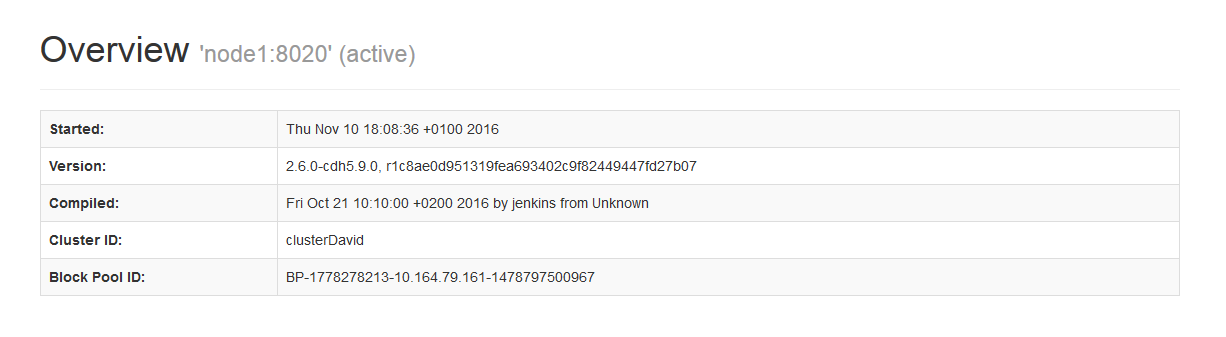
\includegraphics[width=0.9\textwidth]{C:/Users/David/Desktop/TFG/TFGLatex/presentacion/recursos/overview_cluster.png}
\end{frame}

%%%%%%%%%%%%%%%%%%%%%%%%%%%%%%%%%%%%%%%%%%%%%%%%%%%%%%%%%%%%%%%%%%%%%%%%%%%%%%%%%%%%%%%%%%

\begin{frame}[fragile]
\frametitle{YARN v2 (\textit{MapReduce} incluido)}
Lanzamiento de un trabajo \textit{MapReduce} en un \textit{cluster Hadoop}
\begin{lstlisting}[language=bash, numbers=none, frame=single]
$ hadoop jar WordCount.jar WordCount \
  <input_path> <output_path>
\end{lstlisting}
  
En un navegador escribimos: \path{<ip_resource_manager>:8088}\\
\vfill
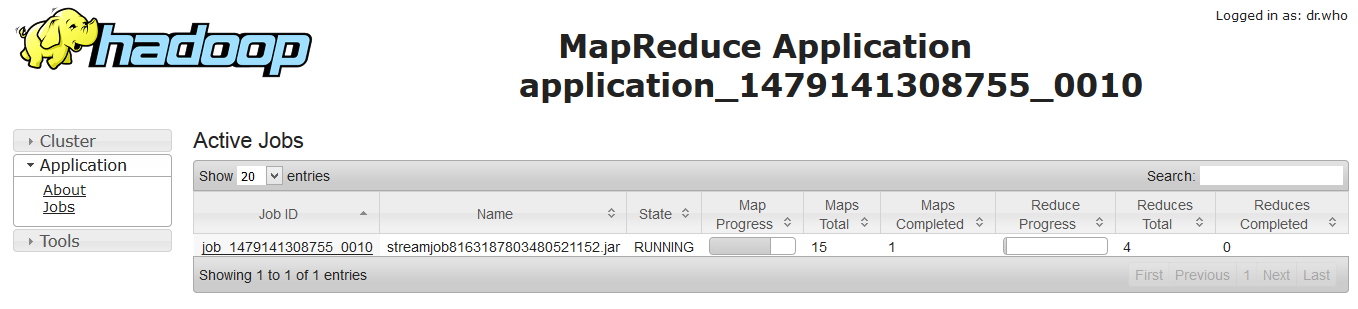
\includegraphics[width=\textwidth]{C:/Users/David/Desktop/TFG/TFGLatex/presentacion/recursos/mapreduce_application.png}
  
\end{frame}

%%%%%%%%%%%%%%%%%%%%%%%%%%%%%%%%%%%%%%%%%%%%%%%%%%%%%%%%%%%%%%%%%%%%%%%%%%%%%%%%%%%%%%%%%%

\subsection{\textit{Spark}}

\begin{frame}[fragile]
\frametitle{\textit{Apache Spark}}

\begin{block}{}
\begin{lstlisting}[language=bash, numbers=none, frame=single]
$ pyspark --master yarn-client
\end{lstlisting}
\end{block}

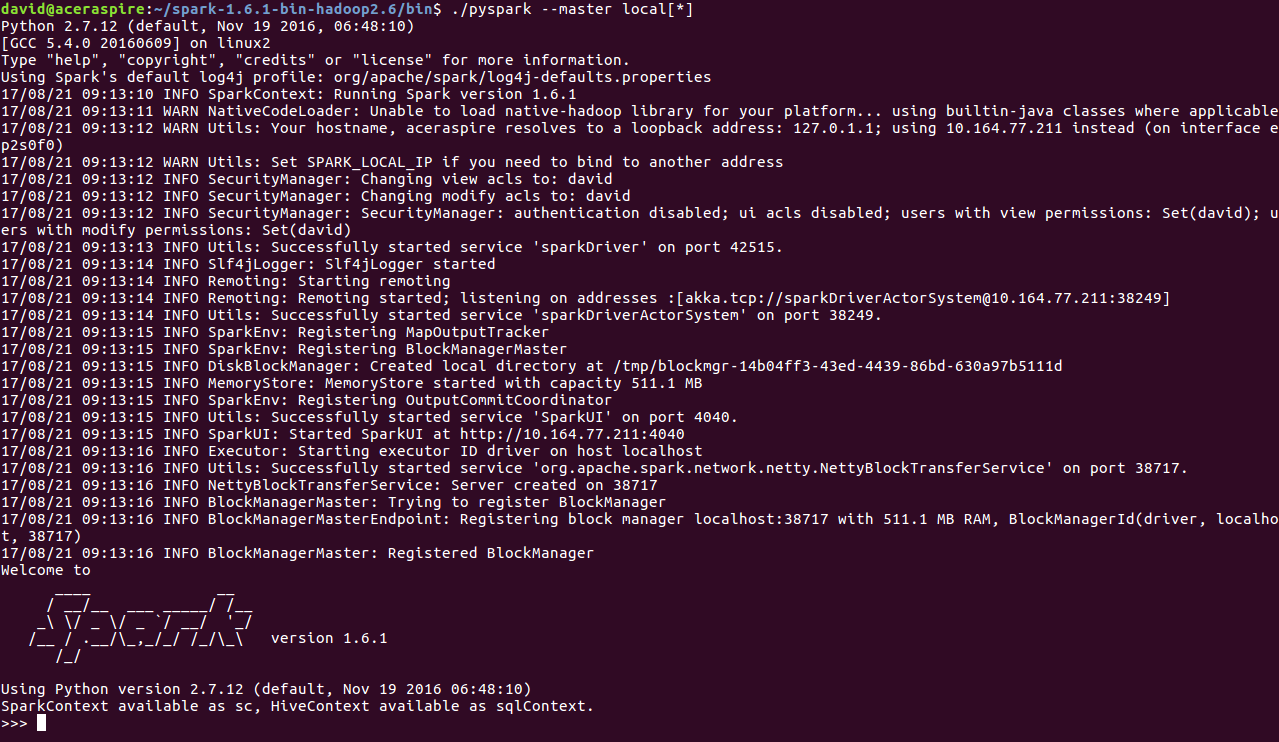
\includegraphics[width=\textwidth]{C:/Users/David/Desktop/TFG/TFGLatex/presentacion/recursos/pyspark_shell.png}

\begin{block}{}
\begin{lstlisting}[language=bash, numbers=none, frame=single, showstringspaces=false]
>>> rdd = sc.parallelize(range(1000))
>>> n = rdd.count()
>>> print("Numero de elementos: ", n)
\end{lstlisting}
\end{block}

\end{frame}

%%%%%%%%%%%%%%%%%%%%%%%%%%%%%%%%%%%%%%%%%%%%%%%%%%%%%%%%%%%%%%%%%%%%%%%%%%%%%%%%%%%%%%%%%%

\begin{frame}
  \frametitle{Cloudera Manager}
  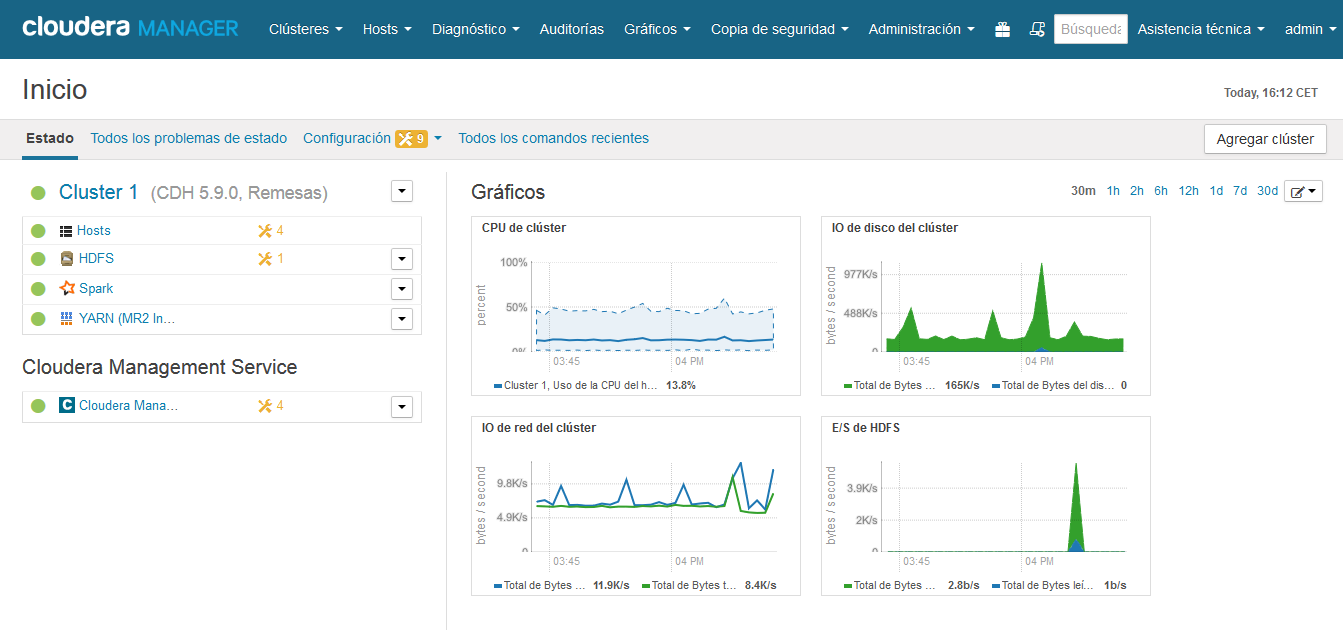
\includegraphics[width=\textwidth]{C:/Users/David/Desktop/TFG/TFGLatex/presentacion/recursos/cloudera_manager.png}
\end{frame}

%%%%%%%%%%%%%%%%%%%%%%%%%%%%%%%%%%%%%%%%%%%%%%%%%%%%%%%%%%%%%%%%%%%%%%%%%%%%%%%%%%%%%%%%%%
%%%%%%%%%%%%%%%%%%%%%%%%%%%%%%%%% MACHINE LEARNING %%%%%%%%%%%%%%%%%%%%%%%%%%%%%%%%%%%%%%%
%%%%%%%%%%%%%%%%%%%%%%%%%%%%%%%%%%%%%%%%%%%%%%%%%%%%%%%%%%%%%%%%%%%%%%%%%%%%%%%%%%%%%%%%%%

\section{\textit{Machine Learning}}

\begin{frame} % machine learning en general
\frametitle{Machine Learning}
\textbf{¿Cómo encaja el machine learning en el Big Data?}
\centering
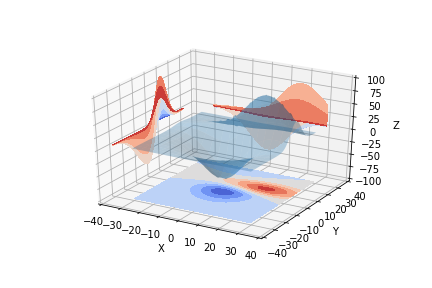
\includegraphics[scale=0.5]{C:/Users/David/Desktop/TFG/TFGLatex/presentacion/recursos/contour_surface.png}
\end{frame}

%%%%%%%%%%%%%%%%%%%%%%%%%%%%%%%%%%%%%%%%%%%%%%%%%%%%%%%%%%%%%%%%%%%%%%%%%%%%%%%%%%%%%%%%%%

\subsection{Algoritmo de \textit{K-Means}}

\begin{frame}[fragile] % contar aprendizaje no supervisado y algoritmo kmeans por encima
\frametitle{Algoritmo de K-Means}

\begin{block}{Características}
  \begin{itemize}
    \item Algoritmo de aprendizaje no supervisado
    \item Clustering
    \item Muy popular y utilizado hoy en día
  \end{itemize}
\end{block}

\begin{block}{Función objetivo}
  $$ J(c, \mu) = \frac{1}{m} \sum_{i=1}^m || x^{(i)} - \mu_{c^{(i)}} ||^2 $$ 
  \centering
  donde $c = (c^{(1)}, \cdots, c^{(m)}) \in \mathds{R}^m$ y $\mu = (\mu_1, \cdots, \mu_k) \in \mathds{R}^k$ \\
  $x^{(i)}, \mu_j \in \mathds{R}^n \quad \forall i=1,\cdots,m; j=1,\cdots,k$
\end{block}

\begin{block}{Código fuente}
\url{https://github.com/davidRetana/TFG}
\end{block}

\end{frame}

%%%%%%%%%%%%%%%%%%%%%%%%%%%%%%%%%%%%%%%%%%%%%%%%%%%%%%%%%%%%%%%%%%%%%%%%%%%%%%%%%%%%%%%%%%

\begin{frame} % kmeans gif
  \animategraphics[loop, controls, width=\linewidth]{1} % {n} cuanto menor mas lento
  {C:/Users/David/Desktop/TFG/TFGLatex/presentacion/recursos/kmeans_imagen}{0}{4}
\end{frame}

%%%%%%%%%%%%%%%%%%%%%%%%%%%%%%%%%%%%%%%%%%%%%%%%%%%%%%%%%%%%%%%%%%%%%%%%%%%%%%%%%%%%%%%%%%

\begin{frame}[fragile] % tabla y grafica comparativa de tiempos (spark vs numpy)
\frametitle{Comparativa de rendimiento}

\begin{table}[!htbp]\small
  \centering
  \begin{tabular}{|c|c|c|c|c|c|} % tabla
    \hline
    & 20kb & 199kb & 1.9mb & 19mb & 198mb \\ \hline
    Python + Sklearn & \textcolor{blue}{$0.020$} & \textcolor{blue}{$0.070$} & \textcolor{blue}{$0.708$} & \textcolor{blue}{$6.585$} & \textcolor{blue}{$65.661$} \\ \hline
    Python + Spark & \textcolor{red}{$1.571$} & \textcolor{red}{$1.672$} & \textcolor{red}{$2.043$} & \textcolor{red}{$7.041$} & \textcolor{red}{$57.577$} \\ \hline
  \end{tabular}
\end{table}

\centering
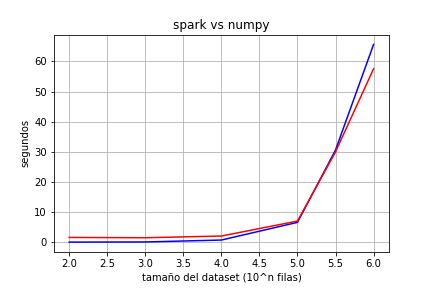
\includegraphics[scale=0.5]{C:/Users/David/Desktop/TFG/TFGLatex/presentacion/recursos/sparkvsnumpy.png}

\end{frame}

%%%%%%%%%%%%%%%%%%%%%%%%%%%%%%%%%%%%%%%%%%%%%%%%%%%%%%%%%%%%%%%%%%%%%%%%%%%%%%%%%%%%%%%%%%

\begin{frame}
\Huge{\centerline{Fin}}
\end{frame}

%%%%%%%%%%%%%%%%%%%%%%%%%%%%%%%%%%%%%%%%%%%%%%%%%%%%%%%%%%%%%%%%%%%%%%%%%%%%%%%%%%%%%%%%%%

\end{document} 